\subsubsection{Диаграммы прецедентов}

Диаграмма прецедентов (диаграмма вариантов использования) – диаграмма, на которой отражены отношения, существующие между актёрами и вариантами использования. Актёрами называют некоторые роли, определенные для разрабатываемого проекта, которые пользователь принимает по отношению к системе. Вариантами использования называют возможные действия, которые пользователь может совершить в контексте роли, которую он представляет.

Основная задача – представлять собой единое средство, дающее возможность заказчику, конечному пользователю и разработчику совместно обсуждать функциональность и поведение системы.

Для отражения модели прецедентов на диаграмме используются:
\begin{enumerate}
	\item[1] Рамки системы (англ. system boundary) – прямоугольник с названием в верхней части и эллипсами (прецедентами) внутри. Часто может быть опущен без потери полезной информации.
	\item[2] Актер (англ. actor) – стилизованный человечек, обозначающий набор ролей пользователя (понимается в широком смысле: человек, внешняя сущность, класс, другая система), взаимодействующего с некоторой сущностью (системой, подсистемой, классом). Актёры не могут быть связаны друг с другом (за исключением отношений обобщения/наследования).
	\item[3] Прецедент – эллипс с надписью, обозначающий выполняемые системой действия (могут включать возможные варианты), приводящие к наблюдаемым актёрами результатам. Надпись может быть именем или описанием (с точки зрения актёров) того, «что» делает система (а не «как»). Имя прецедента связано с непрерываемым (атомарным) сценарием – конкретной последовательностью действий, иллюстрирующей поведение. В ходе сценария актёры обмениваются с системой сообщениями. Сценарий может быть приведён на диаграмме прецедентов в виде UML-комментария. С одним прецедентом может быть связано несколько различных сценариев.
\end{enumerate}

Для проектируемого проекта, диаграмма прецедентов будет иметь следующий вид (рисунок).

\begin{figure}[h!]
	\centering
	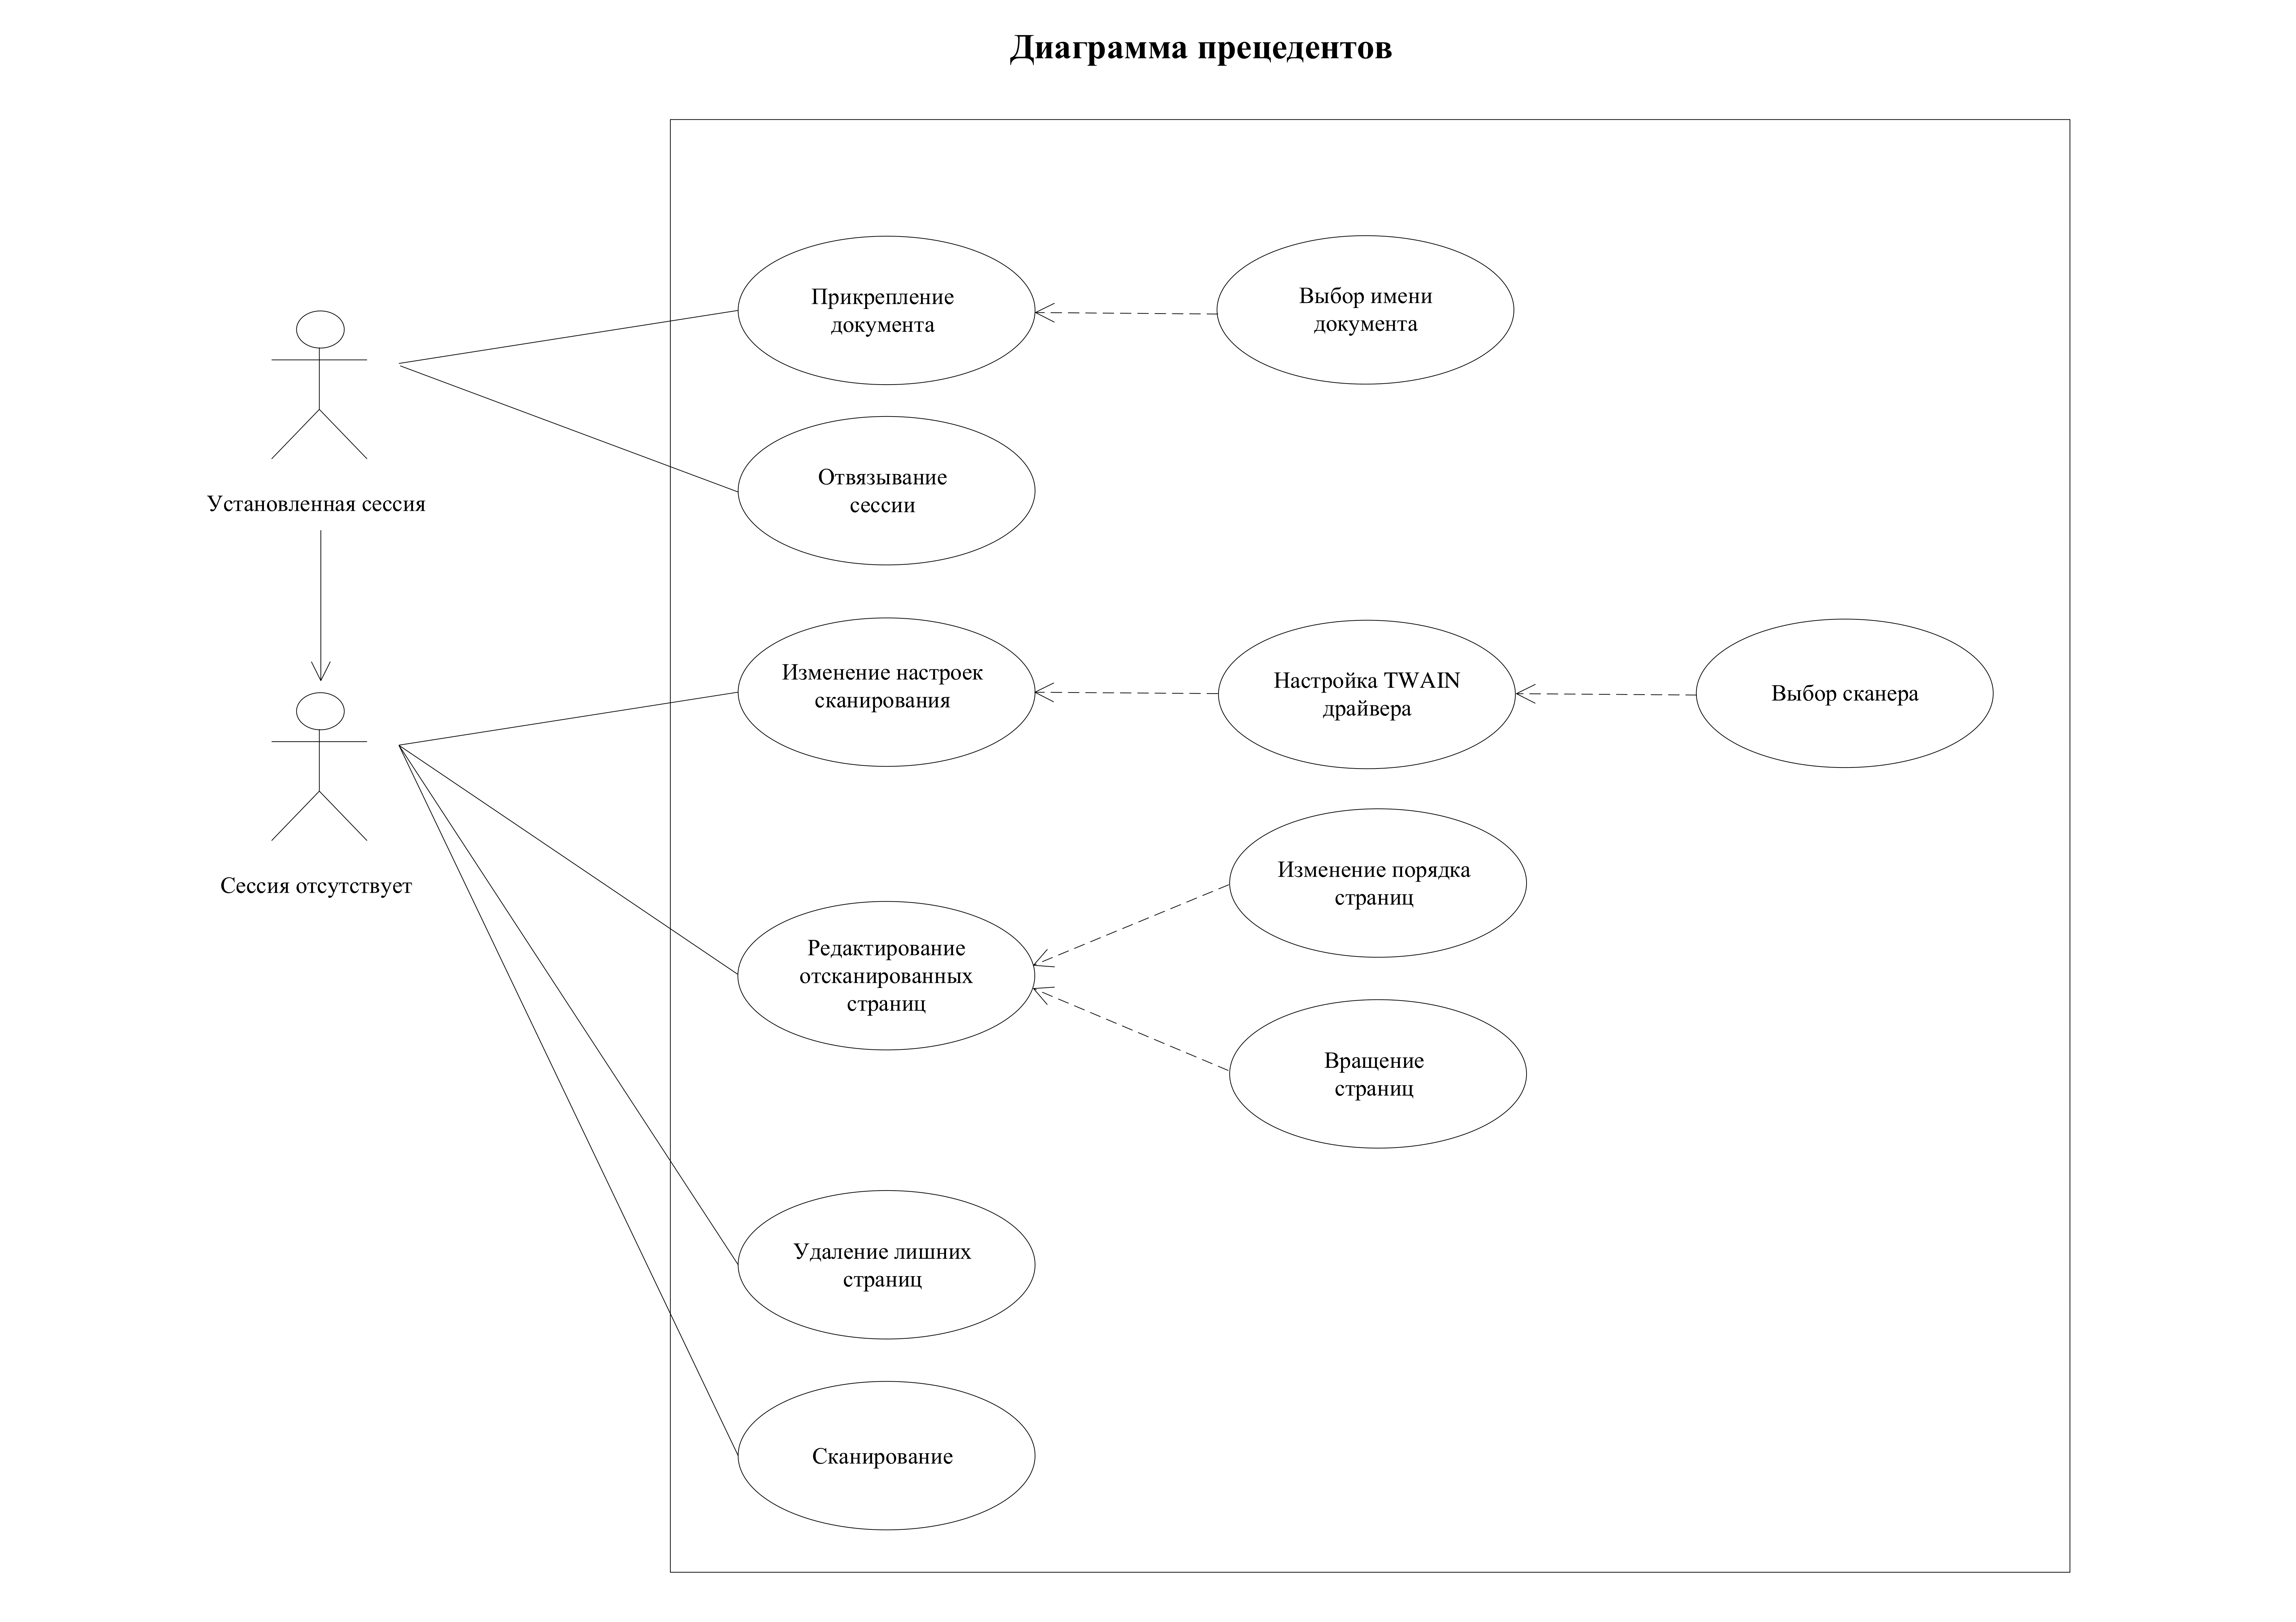
\includegraphics[scale=0.08]{pl2_precendent.png}
	\caption{Диаграмма прецендентов}
\end{figure}

В рамках проектируемого проекта, подразумевается две роли (т.е. два актера):
\begin{enumerate}
	\item[1] Пользователь, который уже привязал сессию СЭД к приложению. Такой пользователь может прикреплять документы на основе привязанной сессии. Так же такой актер может производить все остальные действия, доступные пользователю без сессии.
	\item[2] Пользователь, который не прикрепил сессию. У такого актера есть возможность сканировать документы, редактировать отсканированные документы, но нет права прикреплять документы. Для получения этого права нужно зайти в веб версию СЭД и запустить оттуда сканирование.
\end{enumerate}
